\documentclass[14pt]{extbook}
\usepackage{multicol, enumerate, enumitem, hyperref, color, soul, setspace, parskip, fancyhdr} %General Packages
\usepackage{amssymb, amsthm, amsmath, bbm, latexsym, units, mathtools} %Math Packages
\everymath{\displaystyle} %All math in Display Style
% Packages with additional options
\usepackage[headsep=0.5cm,headheight=12pt, left=1 in,right= 1 in,top= 1 in,bottom= 1 in]{geometry}
\usepackage[usenames,dvipsnames]{xcolor}
\usepackage{dashrule}  % Package to use the command below to create lines between items
\newcommand{\litem}[1]{\item#1\hspace*{-1cm}\rule{\textwidth}{0.4pt}}
\pagestyle{fancy}
\lhead{Progress Quiz 1}
\chead{}
\rhead{Version A}
\lfoot{3114-1073}
\cfoot{}
\rfoot{Fall 2020}
\begin{document}

\begin{enumerate}
\litem{
Solve the equation below. Then, choose the interval that contains the solution.\[ -13(6x + 18) = -4(7x + 17) \]\begin{enumerate}[label=\Alph*.]
\item \( x \in [-3.4, -3.2] \)
\item \( x \in [-3.1, -0.2] \)
\item \( x \in [5.8, 8] \)
\item \( x \in [-7.6, -5.4] \)
\item \( \text{There are no real solutions.} \)

\end{enumerate} }
\litem{
First, find the equation of the line containing the two points below. Then, write the equation as $ y=mx+b $ and choose the intervals that contain $m$ and $b$.\[ (-6, -8) \text{ and } (4, 7) \]\begin{enumerate}[label=\Alph*.]
\item \( m \in [1.5, 8.5] \hspace*{3mm} b \in [2.37, 3.66] \)
\item \( m \in [-4.5, -0.5] \hspace*{3mm} b \in [12.85, 13.98] \)
\item \( m \in [1.5, 8.5] \hspace*{3mm} b \in [-2.24, -1.82] \)
\item \( m \in [1.5, 8.5] \hspace*{3mm} b \in [0.42, 2.34] \)
\item \( m \in [1.5, 8.5] \hspace*{3mm} b \in [-1.93, -0.77] \)

\end{enumerate} }
\litem{
First, find the equation of the line containing the two points below. Then, write the equation as $ y=mx+b $ and choose the intervals that contain $m$ and $b$.\[ (-9, 3) \text{ and } (11, -2) \]\begin{enumerate}[label=\Alph*.]
\item \( m \in [-0.66, 0.07] \hspace*{3mm} b \in [11.99, 12.53] \)
\item \( m \in [-0.66, 0.07] \hspace*{3mm} b \in [-1.67, -0.51] \)
\item \( m \in [-0.66, 0.07] \hspace*{3mm} b \in [-13.53, -11.98] \)
\item \( m \in [-0.15, 1.1] \hspace*{3mm} b \in [-5.62, -4.21] \)
\item \( m \in [-0.66, 0.07] \hspace*{3mm} b \in [0.04, 2.07] \)

\end{enumerate} }
\litem{
Solve the equation below. Then, choose the interval that contains the solution.\[ -12(-13x + 17) = -14(18x -8) \]\begin{enumerate}[label=\Alph*.]
\item \( x \in [-0.16, 0.35] \)
\item \( x \in [0.57, 0.88] \)
\item \( x \in [-1.07, -0.4] \)
\item \( x \in [-0.66, 0.15] \)
\item \( \text{There are no real solutions.} \)

\end{enumerate} }
\litem{
Solve the linear equation below. Then, choose the interval that contains the solution.\[ \frac{-5x -7}{7} - \frac{3x + 7}{2} = \frac{-5x + 5}{8} \]\begin{enumerate}[label=\Alph*.]
\item \( x \in [-3.9, -3] \)
\item \( x \in [-1.9, -1.3] \)
\item \( x \in [-12.1, -11.3] \)
\item \( x \in [0.3, 1.8] \)
\item \( \text{There are no real solutions.} \)

\end{enumerate} }
\litem{
Write the equation of the line in the graph below in Standard form $Ax+By=C$. Then, choose the intervals that contain $A, B, \text{ and } C$.
\begin{center}
    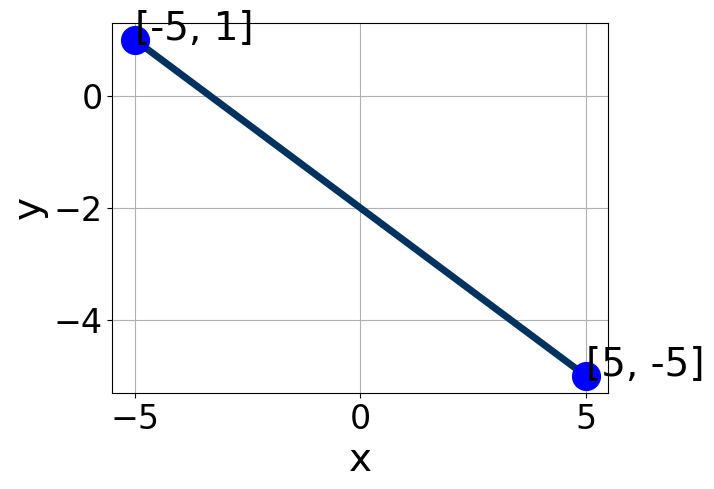
\includegraphics[width=0.5\textwidth]{../Figures/linearGraphToStandardA.png}
\end{center}
\begin{enumerate}[label=\Alph*.]
\item \( A \in [5, 8], \hspace{3mm} B \in [3.8, 5.5], \text{ and } \hspace{3mm} C \in [-18, -14] \)
\item \( A \in [-8, -4], \hspace{3mm} B \in [-5.1, -3.5], \text{ and } \hspace{3mm} C \in [14, 20] \)
\item \( A \in [-0.75, 3.25], \hspace{3mm} B \in [-0.7, 2.3], \text{ and } \hspace{3mm} C \in [-8, -3] \)
\item \( A \in [-0.75, 3.25], \hspace{3mm} B \in [-1.3, 0.6], \text{ and } \hspace{3mm} C \in [-1, 12] \)
\item \( A \in [5, 8], \hspace{3mm} B \in [-5.1, -3.5], \text{ and } \hspace{3mm} C \in [14, 20] \)

\end{enumerate} }
\litem{
Find the equation of the line described below. Write the linear equation as $ y=mx+b $ and choose the intervals that contain $m$ and $b$.\[ \text{Parallel to } 8 x + 5 y = 3 \text{ and passing through the point } (-7, -4). \]\begin{enumerate}[label=\Alph*.]
\item \( m \in [-4.5, -1.3] \hspace*{3mm} b \in [-20.2, -11.2] \)
\item \( m \in [-4.5, -1.3] \hspace*{3mm} b \in [0, 4] \)
\item \( m \in [-0.3, 2.6] \hspace*{3mm} b \in [7.2, 9.2] \)
\item \( m \in [-4.5, -1.3] \hspace*{3mm} b \in [15.2, 16.2] \)
\item \( m \in [-0.8, 0.4] \hspace*{3mm} b \in [-20.2, -11.2] \)

\end{enumerate} }
\litem{
Write the equation of the line in the graph below in Standard form $Ax+By=C$. Then, choose the intervals that contain $A, B, \text{ and } C$.
\begin{center}
    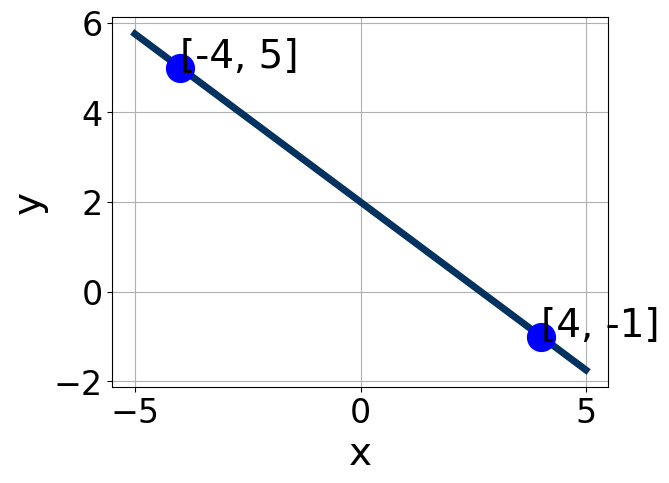
\includegraphics[width=0.5\textwidth]{../Figures/linearGraphToStandardCopyA.png}
\end{center}
\begin{enumerate}[label=\Alph*.]
\item \( A \in [-1.6, 1], \hspace{3mm} B \in [0.3, 1.2], \text{ and } \hspace{3mm} C \in [-2.2, -0.3] \)
\item \( A \in [2.4, 4.9], \hspace{3mm} B \in [-4.6, -3.3], \text{ and } \hspace{3mm} C \in [7.2, 8.8] \)
\item \( A \in [2.4, 4.9], \hspace{3mm} B \in [2.2, 5.4], \text{ and } \hspace{3mm} C \in [-10.2, -7.9] \)
\item \( A \in [-1.6, 1], \hspace{3mm} B \in [-2.2, 0.6], \text{ and } \hspace{3mm} C \in [0.3, 2.2] \)
\item \( A \in [-5, -2], \hspace{3mm} B \in [2.2, 5.4], \text{ and } \hspace{3mm} C \in [-10.2, -7.9] \)

\end{enumerate} }
\litem{
Find the equation of the line described below. Write the linear equation as $ y=mx+b $ and choose the intervals that contain $m$ and $b$.\[ \text{Perpendicular to } 8 x + 9 y = 3 \text{ and passing through the point } (-7, 3). \]\begin{enumerate}[label=\Alph*.]
\item \( m \in [0.97, 1.96] \hspace*{3mm} b \in [-11.26, -10.86] \)
\item \( m \in [0.97, 1.96] \hspace*{3mm} b \in [9.6, 10.7] \)
\item \( m \in [-1.15, -0.83] \hspace*{3mm} b \in [-5.93, -4.66] \)
\item \( m \in [0.31, 1.03] \hspace*{3mm} b \in [10.52, 11.26] \)
\item \( m \in [0.97, 1.96] \hspace*{3mm} b \in [10.52, 11.26] \)

\end{enumerate} }
\litem{
Solve the linear equation below. Then, choose the interval that contains the solution.\[ \frac{7x -9}{4} - \frac{5x -8}{2} = \frac{-6x -6}{5} \]\begin{enumerate}[label=\Alph*.]
\item \( x \in [-12.11, -9.11] \)
\item \( x \in [-4.37, 0.63] \)
\item \( x \in [-8.56, -4.56] \)
\item \( x \in [8.22, 18.22] \)
\item \( \text{There are no real solutions.} \)

\end{enumerate} }
\end{enumerate}

\end{document}